\documentclass[tikz,border=5mm]{standalone}
\usepackage[T1]{fontenc}
\usepackage{fontspec}
\setmainfont{Fira Sans}[
  BoldFont=Fira Sans Bold,
  ItalicFont=Fira Sans Italic,
]
\usetikzlibrary{positioning, arrows.meta, shadows.blur, calc, shapes.geometric}

\definecolor{mTeal}{HTML}{2B7A78}
\definecolor{mBrown}{HTML}{C9956B}
\definecolor{mGray}{HTML}{888888}
\definecolor{mBg}{HTML}{FAFAFA}

\begin{document}
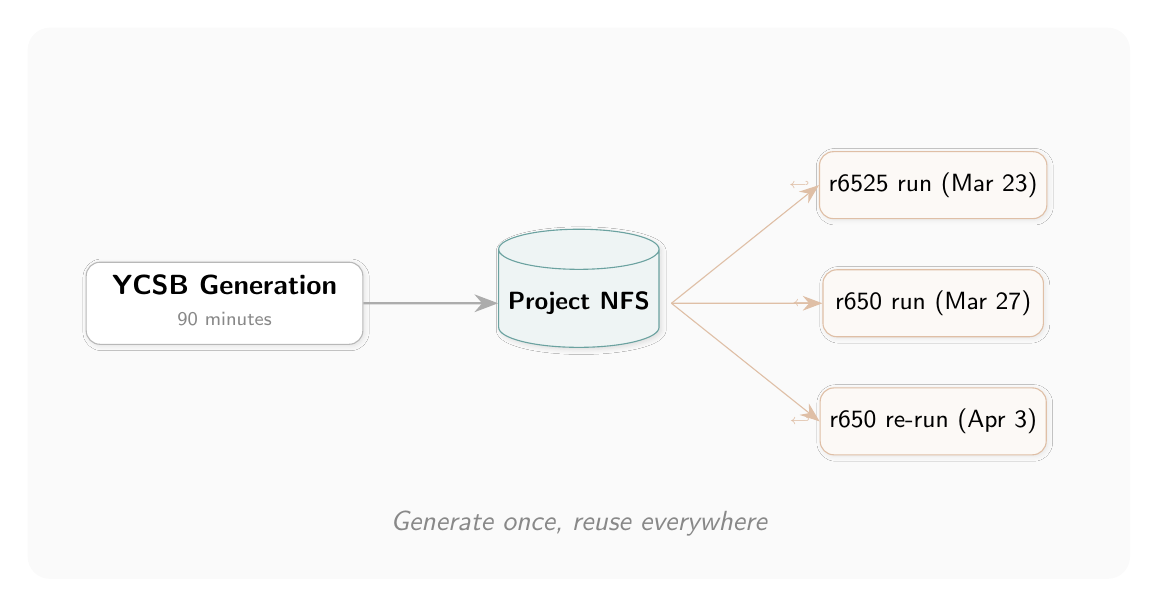
\begin{tikzpicture}[
  every node/.style={font=\sffamily},
  box/.style={draw=mGray!50, fill=white, rounded corners=5pt,
              minimum width=2.8cm, minimum height=1cm,
              blur shadow={shadow blur steps=5, shadow xshift=0.2mm,
              shadow yshift=-0.2mm, shadow opacity=10}},
  run/.style={draw=mBrown!60, fill=mBrown!6, rounded corners=5pt,
              minimum width=2.8cm, minimum height=0.85cm, font=\sffamily\small,
              blur shadow={shadow blur steps=4, shadow xshift=0.2mm,
              shadow yshift=-0.2mm, shadow opacity=8}},
  >=Stealth,
]
  \fill[mBg, rounded corners=8pt] (-7,-3.5) rectangle (7,3.5);

  % Generation box
  \node[box, draw=mGray!60] (gen) at (-4.5,0) {
    \begin{tabular}{c}
      \textbf{YCSB Generation}\\[-1pt]
      {\color{mGray}\scriptsize 90 minutes}
    \end{tabular}
  };

  % NFS cylinder
  \node[cylinder, draw=mTeal!70, fill=mTeal!8, shape border rotate=90,
        minimum width=2cm, minimum height=1.5cm, aspect=0.25,
        font=\sffamily\small\bfseries,
        blur shadow={shadow blur steps=6, shadow xshift=0.3mm,
        shadow yshift=-0.3mm, shadow opacity=12}] (nfs) at (0,0) {Project NFS};

  % Experiment runs
  \node[run] (r1) at (4.5, 1.5) {r6525 run (Mar 23)};
  \node[run] (r2) at (4.5, 0) {r650 run (Mar 27)};
  \node[run] (r3) at (4.5,-1.5) {r650 re-run (Apr 3)};

  % Link icons
  \foreach \r in {r1,r2,r3} {
    \node[mBrown!60, font=\tiny] at ($(\r.west)+(-0.25,0)$) {$\hookleftarrow$};
  }

  % Arrows
  \draw[-{Stealth[length=3mm]}, thick, mGray!70] (gen.east) -- (nfs.west);
  \draw[-{Stealth[length=2.5mm]}, mBrown!60] (nfs.east) ++(0.15,0) -- (r1.west);
  \draw[-{Stealth[length=2.5mm]}, mBrown!60] (nfs.east) ++(0.15,0) -- (r2.west);
  \draw[-{Stealth[length=2.5mm]}, mBrown!60] (nfs.east) ++(0.15,0) -- (r3.west);

  % Tagline
  \node[mGray, font=\sffamily\itshape] at (0,-2.8) {Generate once, reuse everywhere};
\end{tikzpicture}
\end{document}
